\documentclass[11pt,letterpaper]{article}
\usepackage[margin=1.04in,headheight=15pt]{geometry}
\usepackage[T1]{fontenc}
\usepackage[utf8]{inputenc}
\usepackage{lmodern,microtype,amsmath,amssymb,amsthm,mathtools,mathrsfs,stmaryrd}
\usepackage{enumitem,booktabs,array,longtable,tabularx,xcolor,tikz}
\usetikzlibrary{arrows.meta,positioning,calc,shapes.geometric,fit}
\usepackage[colorlinks=true,linkcolor=black,urlcolor=black,citecolor=black]{hyperref}
\hypersetup{pdftitle={Formal Self-Awareness in Semi-Ideal Computers},pdfauthor={<Brian Tenneson>},pdfsubject={Expanded mathematical research draft on semi-ideal computers and self-theories}}
\usepackage{fancyhdr}
\pagestyle{fancy}\fancyhf{}\lhead{Formal Self-Awareness in Semi-Ideal Computers}\rhead{Research Draft 0.1}\cfoot{\thepage}
\setlength{\parindent}{1.1em}\setlength{\parskip}{.25em}
\setlist{leftmargin=2.1em, itemsep=.24em, topsep=.3em}
\newtheorem{theorem}{Theorem}[section]
\newtheorem{lemma}[theorem]{Lemma}
\newtheorem{proposition}[theorem]{Proposition}
\newtheorem{corollary}[theorem]{Corollary}
\newtheorem{claim}[theorem]{Claim}
\theoremstyle{definition}\newtheorem{definition}[theorem]{Definition}\newtheorem{example}[theorem]{Example}\newtheorem{protocol}[theorem]{Protocol}\newtheorem{question}[theorem]{Open Problem}
\theoremstyle{remark}\newtheorem{remark}[theorem]{Remark}
\newcommand{\N}{\mathbb N}\newcommand{\Pset}{\mathcal P}\newcommand{\Con}{\operatorname{Con}}
\newcommand{\Sent}{\operatorname{Sent}}
\newcommand{\Th}{\operatorname{Th}}
\newcommand{\Self}{\operatorname{Self}}
\newcommand{\SD}{\operatorname{SD}}
\newcommand{\Reach}{\operatorname{Reach}}
\newcommand{\Proof}{\operatorname{Proof}}
\newcommand{\Cert}{\operatorname{Cert}}
\newcommand{\Obs}{\operatorname{Obs}}
\newcommand{\Tag}{\operatorname{Tag}}
\newcommand{\lev}{\operatorname{lev}}
\newcommand{\Prov}{\operatorname{Pr}}
\newcommand{\Hist}{\operatorname{Hist}}
\newcommand{\Cost}{\operatorname{Cost}}
\newcommand{\clksim}{\preceq_{\mathrm{clk}}}
\newcommand{\sas}{\preceq_{\mathrm{SA}}}
\newcommand{\tick}{\textsf{tick}}
\newcommand{\source}{\textsf{Source}}
\newcommand{\newpart}{\textsf{Development}}
\newcommand{\cond}{\textsf{Conditional}}
\newcommand{\openstatus}{\textsf{Open}}
\newcommand{\Mtag}{\langle M\rangle}
\newcommand{\Nth}{\N_{>0}}
\newcommand{\qname}[1]{\ulcorner #1\urcorner}
\newcommand{\boxednote}[1]{\begin{center}\fbox{\begin{minipage}{.91\linewidth}#1\end{minipage}}\end{center}}
\title{\bfseries Formal Self-Awareness in Semi-Ideal Computers\\[3pt]
\large Self-Theories, Reflection Depth, Simulation, and Certified Histories\\[6pt]
\normalsize A development of \emph{Self-Awareness} in the language of \emph{Depths of a Simulation}}
\author{\textless{}Brian Tenneson\textgreater{}}
\date{Expanded research draft 0.1 --- October 28, 2026}
\begin{document}
\maketitle
\begin{abstract}
The two-page draft \emph{Self-Awareness} proposes internal representations, a tagging operator, self-models, self-descriptive formulas, and the self-theory of an automated theorem prover (ATP). This manuscript develops those definitions inside Tenneson's $xyz$ formal systems, semi-ideal computers (SICs), and clocked deterministic simulation preorder. We distinguish naming, self-ascription, verified self-description, internal provability soundness, and reflection depth. A precisely defined syntactic class replaces informal appeals to the ``intended subject'' of a sentence. The resulting reflection hierarchy has finite and $\omega$ examples, a cumulativity theorem under provability soundness, and a non-degenerate rule-driven $\omega$ construction under an explicit proof-generation schema. We define an admissible self-awareness preorder and prove transfer and clocked-hitting-time results only under the necessary tag, quotation, certificate, and timing hypotheses. Optional nondeterministic, cooperative, and history-quotient extensions are stated separately. These are mathematical properties of formal systems, not claims about subjective consciousness, intelligence, or machines that have actually been implemented or tested. Source-derived claims, new developments, and open obligations are identified throughout.
\end{abstract}
\noindent\textbf{Status.} Research expansion for review. No independent machine-checked proof, empirical performance claim, or authorization for publication is asserted. The original two-page draft is treated as the starting text, not silently replaced as a historical source.
\tableofcontents
\clearpage

\section{Introduction: what is the claim?}
The question is not whether a computer feels as humans do. It is whether a computer can express, derive, and correctly certify mathematically meaningful statements whose subject is the computer itself. A machine may contain a name for itself, yet know nothing about the named object; it may assert an impressive fact about itself, yet have no justification; or it may exhibit a finite derivation that a separately specified verifier accepts. These situations must not be conflated.

\emph{Self-Awareness} begins from the simulation framework of \emph{Depths of a Simulation} and defines an internal representation of an ATP $T$, a tagging map $\Tag:T\mapsto\langle T\rangle$, a self-model, and the set $\Self(T)$ of provable self-descriptive sentences. It then lists eight destinations for future work: properties, reflection, predicates, depth, preorder, deterministic/nondeterministic transfer, Tegmark's self-aware substructures, and open problems. The present manuscript follows those eight destinations while adding the qualifications required to make their claims precise.

\paragraph{Guiding question.} When does a computation exhibit a \emph{certified self-description}, and how is that property preserved---or destroyed---by simulation, scheduling, changes of notation, and compression of history?

\paragraph{Roadmap.} Sections 2--3 establish the $xyz$ and SIC foundations and the syntactic notion of a self-theory. Sections 4--6 construct and examine a graded reflection hierarchy. Sections 7--8 develop two different simulation relations, with quantitative depth and time. Sections 9--10 address branching and certified histories. Sections 11--12 test the definitions against minimal examples and connect them to cooperative ATPs. Sections 13--14 state philosophical boundaries and a sharply delimited research agenda.

\subsection{Provenance and status convention}
We call a claim \emph{inherited} when its definitions or proof pattern occur in the corrected \emph{Depths of a Simulation \& Formalized Self-Awareness} core reproduced in the crossover research draft. We call a statement a \emph{development} when this paper adds a definition, example, proof, or stricter operational interface. A conditionally proved theorem is not an unconditional theorem, and a paper-level proof is not an external verifier receipt. Earlier corrected passages take priority over their retained documentary facsimiles.

\section{The $xyz$ language and the SIC layer}
\subsection{Formal consequence and proof length}
\begin{definition}[$xyz$ formal system]
An $xyz$ formal system is $F=(x,y,z)$, where $x$ is a nonempty alphabet, $y$ is a collection of finite well-formed strings, and $z$ is a family of finitary partial inference rules $r:y^k\rightharpoonup y$. For $\Gamma\subseteq y$, write $\Gamma\vdash_F\varphi$ if a finite legal derivation of $\varphi$ exists from $\Gamma$, and
\[
\Con_F(\Gamma)=\{\varphi\in y:\Gamma\vdash_F\varphi\}.
\]
\end{definition}
Premises are available without a primitive inference application. Let $h_F(\Gamma,\varphi)$ denote the minimum number of primitive inference applications in a derivation, or $\infty$ if $\varphi$ is not derivable. When comparing with a source's length-of-proof convention $\|\varphi\|_F(\Gamma)$, that convention must be fixed before an equality is asserted.

\subsection{Semi-ideal computers}
\begin{definition}[SIC; inherited six axioms]
For $Y\subseteq y$ a semi-ideal computer over $Y$ is $M=(C_M,H_M)$, where
\[
C_M:\Pset(Y)\times\Nth\to\Pset(Y),\qquad
H_M:\Pset(Y)\times\Nth\to\{0,1\},
\]
and, for every $\Gamma\subseteq Y$ and $m\in\Nth$,
\begin{align*}
C_M(\Gamma,1)&=\Gamma,\\
C_M(\Gamma,m)&\subseteq C_M(\Gamma,m+1),\\
H_M(\Gamma,m)=1&\Longrightarrow H_M(\Gamma,m+1)=1,\\
H_M(\Gamma,m)=1&\Longrightarrow C_M(\Gamma,m+1)=C_M(\Gamma,m).
\end{align*}
The first two type clauses together with the four displayed behavioral clauses form the six SIC requirements. The state space is $S_M=\Pset(Y)$, since every $\Gamma$ is a stage-one state.
\end{definition}
\begin{remark}[What a SIC is not]
Monotone stage evolution does not itself imply that each new formula is logically valid, that any proof was searched for, or that the halting bit indicates finding a designated theorem. These require additional hypotheses. In particular, do not mistake $H_M(\Gamma,m)=1$ for a claim that $M$ has proved a sentence \emph{about itself}.
\end{remark}
\begin{definition}[ATP and rule-driven ATP]
An ATP is a SIC intended to enumerate derivable formulas or to search for selected targets. An \emph{enumerating ATP} satisfies $\bigcup_{m\ge1}C_M(\Gamma,m)=\Con_F(\Gamma)\cap Y$ on its declared inputs. A SIC is \emph{rule-driven} if each member added at stage $m+1$ is a direct consequence of the preceding stage.
\end{definition}
\begin{definition}[Operational theorem set at a designated input]
A \emph{tagged presentation} of an ATP includes a distinguished input $A_M\subseteq Y$ and a fixed ambient calculus. Write
\[
\Th_M(A_M):=\bigcup_{m\ge1}C_M(A_M,m).
\]
The shorthand $M\vdash_A\varphi$ means $\varphi\in\Th_M(A_M)$. It is an \emph{operational output assertion}; the stronger phrase ``certifiably proves'' is reserved for a supplied certificate accepted by the declared verifier. If $\Th_M(A_M)\subseteq\Con_F(A_M)$, we call the output deductively sound at $A_M$.
\end{definition}
\begin{proposition}[Rule-driven soundness of outputs]\label{prop:sound}
If $M$ is rule-driven over $F$, then $\Th_M(A_M)\subseteq\Con_F(A_M)$.
\end{proposition}
\begin{proof}
Induct on $m$. At stage one the formulas are premises from $A_M$. If each formula in stage $m$ is derivable from $A_M$, a newly added formula at $m+1$ is obtained by a legal finitary rule from those formulas, so is also derivable. The union of stages is therefore contained in the consequence set.
\end{proof}
Soundness of ordinary formal consequence is \emph{not} identical with truth of an interpretation of the special predicates $\operatorname{ATP}$ or $\Prov$; their meanings will be stipulated separately.

\section{Internal representations and self-theories}
\subsection{Naming a machine is not running it}
\begin{definition}[Internal representation and tag; preserved]
For a tagged ATP $M$, $\Mtag$ is a designated closed term in its accompanying language $L_M$ that denotes the presented machine. A tagging operator assigns $\Tag(M)=\Mtag$. The name may be a primitive symbolic tag, a quoted term, a canonical description, or a G\"odel code, provided the chosen naming semantics is declared.
\end{definition}
A tag is a term, not a copy of the transition function. No arithmetization is compulsory. However, the mere existence of a term $\Mtag$ does not establish that its denotation is $M$: that identification is a \emph{correctness assumption} about the presentation.
\begin{definition}[Faithful designation]
A tag is \emph{faithful} in an interpretation $\mathfrak A$ if the denotation function satisfies $\llbracket\Mtag\rrbracket_{\mathfrak A}=M$. Tag faithfulness and object-language ability to \emph{prove} faithfulness are different properties.
\end{definition}

\subsection{Replacing intended meaning with declared syntax}
\begin{definition}[Self-descriptive syntactic class]
For each tagged presentation, fix a syntactically recognizable class $\SD_M\subseteq\Sent(L_M)$ of sentences with a designated subject position occupied by $\Mtag$. Require
\[
\operatorname{ATP}(\Mtag)\in\SD_M,
\quad
\Prov(\Mtag,\qname{\varphi})\in\SD_M,
\]
whenever the latter is well formed. Other predicates, such as $\operatorname{Halts}$ or $\operatorname{UsesRule}$, count only when their syntax declares the machine argument to be the subject. A sentence that merely contains $\Mtag$ in an incidental argument position need not be self-descriptive.
\end{definition}
This is the corrected source convention. A purely semantic phrase such as ``intended subject'' is not enough to establish the properties of a syntactic class or of a translation of languages.
\begin{definition}[Self-theory; source definition made explicit]
The self-theory of a tagged ATP on $A_M$ is
\[
\boxed{\Self_A(M)=\Th_M(A_M)\cap\SD_M.}
\]
The \emph{self-model} is the pair $\operatorname{SelfModel}_A(M)=(\Mtag,\Self_A(M))$ together with the declared interpretations of the self-descriptive predicates. The last semantic component is needed to distinguish correct description from mere assertion.
\end{definition}
\begin{proposition}[Elementary self-theory properties]
For every tagged ATP, (i) $\Self_A(M)\subseteq\Th_M(A_M)$; (ii) $\Self_A(M)=\varnothing$ iff $M$ emits no declared self-descriptive formula on $A_M$; and (iii) if $M\vdash_A\operatorname{ATP}(\Mtag)$ then $\Self_A(M)\ne\varnothing$.
\end{proposition}
\begin{proof}
The first two statements follow from the definition as an intersection. The third follows from the specified inclusion $\operatorname{ATP}(\Mtag)\in\SD_M$.
\end{proof}
\begin{remark}[An important non-implication]
From $\operatorname{ATP}(\Mtag)\in\Self_A(M)$ one \emph{cannot} infer that the machine verified its own ATP axioms or even established the claim semantically. It may have received the formula as a premise.
\end{remark}

\begin{figure}[htbp]
\centering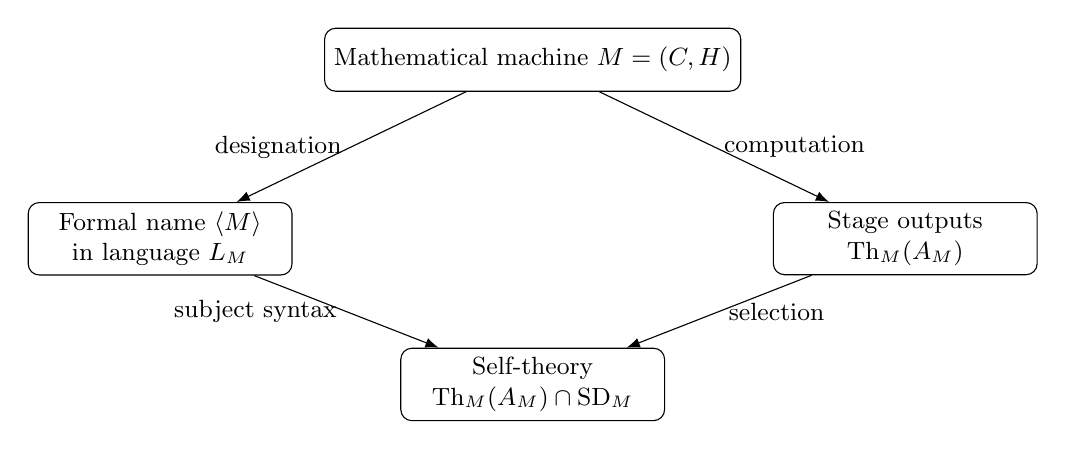
\begin{tikzpicture}[node distance=1.3cm,>=Latex,every node/.style={font=\small},box/.style={draw,rounded corners,align=center,minimum width=3.35cm,minimum height=.8cm}]
\node[box] (m) {Mathematical machine $M=(C,H)$};
\node[box,below left=1.4cm and .4cm of m] (tag) {Formal name $\langle M\rangle$\\in language $L_M$};
\node[box,below right=1.4cm and .4cm of m] (work) {Stage outputs\\$\Th_M(A_M)$};
\node[box,below=3.25cm of m] (self) {Self-theory\\$\Th_M(A_M)\cap\SD_M$};
\draw[->] (m) -- node[left]{designation} (tag);
\draw[->] (m) -- node[right]{computation} (work);
\draw[->] (tag) -- node[left]{subject syntax} (self);
\draw[->] (work) -- node[right]{selection} (self);
\end{tikzpicture}
\caption{A name, a stream of outputs, and a self-theory are different mathematical objects.}
\end{figure}

\subsection{Changing the tag}
\begin{proposition}[Renaming invariance with explicit conditions]\label{prop:rename}
Suppose two tagged presentations of the same underlying ATP are related by a bijective, arity-preserving renaming $\tau$ commuting with formula formation and quotation, satisfying $\tau(\Mtag)=\langle M\rangle'$ and $\tau[\SD_M]=\SD'_M$, and sending the output theory onto the renamed output theory. Then
\[
\tau[\Self_A(M)]=\Self_A'(M).
\]
\end{proposition}
\begin{proof}
An injective map distributes over intersection when its inverse is defined on the two images. Apply $\tau$ to $\Th_M(A_M)\cap\SD_M$ and use the two set-image equalities from the hypotheses.
\end{proof}
A many-to-one renaming can identify distinct predicates or formulas and is not covered by this proposition.

\section{Awareness predicates and the first examples}
\begin{definition}[Minimal formal self-identification]
An ATP has \emph{Level 1 self-identification} on $A_M$ if it has a faithful tag and $M\vdash_A\operatorname{ATP}(\Mtag)$. \emph{Level 0}, relative to this base test, means that no such verified output assertion occurs.
\end{definition}
\begin{example}[The premise-handed machine]\label{ex:handed}
Take $Y=\{p\}$ with $p=\operatorname{ATP}(\Mtag)$, and set $C_M(\Gamma,m)=\Gamma$, $H_M(\Gamma,m)=0$. Fix $A_M=\{p\}$. This is a SIC: it starts from $\Gamma$, never shrinks or halts, and never changes. It outputs $p$, so has Level 1 by the weak criterion. However, it made no inference and learned nothing about its own implementation. This is a \emph{degenerate self-ascription}, not a discovered self-proof.
\end{example}
\begin{example}[One genuinely derived self-description]\label{ex:derived}
Let $A_M=\{a\}$, let $p=\operatorname{ATP}(\Mtag)$, and let the formal calculus have a declared legal rule $r(a)=p$. Define
\[
C_M(\Gamma,1)=\Gamma,\qquad
C_M(\Gamma,m)=\Gamma\cup\{p:a\in\Gamma\}\quad(m\ge2),\qquad H_M=0.
\]
This is a rule-driven SIC and $p\notin A_M$; on $A_M$ the self-description first appears at stage 2. It is a derivation of $p$ \emph{from the stated rule and premise}, not yet a proof that $p$ correctly describes the implementation. That final semantic step needs a faithful specification of the rule and machine.
\end{example}
\begin{definition}[Certified self-description]
A self-descriptive formula $\psi\in\SD_M$ is \emph{certified at stage $m$} if the operational record contains a finite certificate $\pi$ that an independent verifier $V_F$ accepts as a derivation $A_M\vdash_F\psi$ and if $\psi$ appears in the accepted stage-$m$ output. It is \emph{semantically certified} when the formal interpretation also validates the advertised property of the tagged implementation.
\end{definition}
\begin{remark}[Two trust boundaries]
Verifier acceptance establishes formal derivability relative to $F$ and $A_M$; semantic certification additionally requires that the adopted axioms, tags, and operational predicate interpretations apply to the actual machine. A checker does not magically turn a false specification into a true one.
\end{remark}

\section{Quotation, provability, and the reflection sequence}
\subsection{The internal provability predicate}
\begin{definition}[Names for formulas and $\Prov$]
Assume a quotation function $\varphi\mapsto\qname{\varphi}$ assigning different names to different formulas. The language has a primitive binary predicate $\Prov$, intended to express
\[
\Prov(\Mtag,\qname{\varphi})\quad\text{``the tagged ATP proves $\varphi$ on $A_M$''.}
\]
Quotation need not be numeric. The intended semantics does not itself grant a formal derivation of every true provability sentence.
\end{definition}
The choice between (i) $A_M\vdash_F\varphi$, (ii) $M\vdash_A\varphi$, and (iii) verifier-accepted proof of $\varphi$ \emph{matters}. In this paper $\Prov$ refers to the designated operational output relation unless a different interpretation is explicitly specified; when $M$ is deductively effective and sound, (i) and (ii) coincide. This prevents an equivocation between logical theoremhood and an implementation's discovery history.
\begin{definition}[Reflection sequence]
For a tagged ATP whose language contains the required quotations, define
\[
\theta_0^M:=\operatorname{ATP}(\Mtag),\qquad
\theta_{k+1}^M:=\Prov(\Mtag,\qname{\theta_k^M})\quad(k\ge0).
\]
The first three layers read ``I am an ATP,'' ``I prove that I am an ATP,'' and ``I prove that I prove that I am an ATP.''
\end{definition}
\begin{proposition}[Syntactic distinctness]\label{prop:distinct}
If $\operatorname{ATP}$ and $\Prov$ are distinct predicate symbols and quotation is injective, the formulas $\theta_0^M,\theta_1^M,\dots$ are pairwise distinct.
\end{proposition}
\begin{proof}
The first formula has leading predicate $\operatorname{ATP}$ and every successor has leading predicate $\Prov$. If $\theta_{j+1}^M=\theta_{k+1}^M$, equality of the second argument yields $\qname{\theta_j^M}=\qname{\theta_k^M}$; injectivity reduces equality to the preceding indices. Iterating reaches the differing leading predicates unless $j=k$.
\end{proof}
\begin{definition}[Levels and spectrum]
Set
\[
\mathcal L(M):=\{n\in\Nth:M\vdash_A\theta_{n-1}^M\},\qquad
\lev(M):=\sup\mathcal L(M)\in\N\cup\{\omega\},
\]
where $\sup\varnothing=0$. The $n$th reflection level is attained when $n\in\mathcal L(M)$. A system has \emph{level $\omega$} if its achieved reflection levels are unbounded. Under provability soundness, Theorem~\ref{thm:cum} shows that this is equivalent to attaining every finite reflection level. Here $\omega$ means the supremum of the finite hierarchy, not an assertion of omniscience.
\end{definition}

\begin{figure}[htbp]\centering
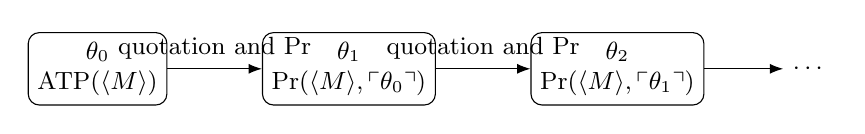
\begin{tikzpicture}[>=Latex, every node/.style={font=\small}, b/.style={draw,rounded corners,minimum height=.68cm,align=center}]
\node[b] (a) {$\theta_0$\\$\operatorname{ATP}(\langle M\rangle)$};
\node[b,right=1.2cm of a] (b) {$\theta_1$\\$\Pr(\langle M\rangle,\ulcorner\theta_0\urcorner)$};
\node[b,right=1.2cm of b] (c) {$\theta_2$\\$\Pr(\langle M\rangle,\ulcorner\theta_1\urcorner)$};
\node[right=1cm of c] (d) {$\cdots$};
\draw[->] (a)--node[above]{quotation and $\Pr$} (b);
\draw[->] (b)--node[above]{quotation and $\Pr$} (c);
\draw[->] (c)--(d);
\end{tikzpicture}
\caption{The finite reflection ladder is a sequence of sentences. Merely forming a sentence is not proving it.}
\end{figure}

\subsection{Truthful self-ascription versus unearned self-ascription}
\begin{definition}[Provability soundness and internal necessitation]
A tagged ATP is \emph{provability sound} on $A_M$ if
\[
M\vdash_A\Prov(\Mtag,\qname{\varphi})\ \Longrightarrow\ M\vdash_A\varphi
\]
for each formula $\varphi$ in the declared domain. It has \emph{internal necessitation} if the converse implication holds for every such $\varphi$.
\end{definition}
These are separate properties. A primitive provability predicate can be unsound, and an otherwise sound machine can fail to derive true statements about which formulas it has proved.
\begin{example}[Level 2 without Level 1]
Take $Y=\{\theta_0,\theta_1\}$, $A_M=\{\theta_1\}$, and a static SIC $C(\Gamma,m)=\Gamma$, $H=0$. Then $\mathcal L(M)=\{2\}$: the machine asserts ``I prove $\theta_0$'' but does not output $\theta_0$. In the declared operational interpretation this instance of $\Prov$ is false. The example satisfies SIC axioms but not provability soundness.
\end{example}
\begin{theorem}[Cumulativity under provability soundness]\label{thm:cum}
For a provability-sound tagged ATP, $n+1\in\mathcal L(M)$ implies $n\in\mathcal L(M)$. Thus $\mathcal L(M)$ is an initial segment of $\Nth$; if its supremum is finite $k$, then $\mathcal L(M)=\{1,\dots,k\}$.
\end{theorem}
\begin{proof}
If $n+1\in\mathcal L(M)$ then $M\vdash_A\theta_n^M$, which is $\Prov(\Mtag,\qname{\theta_{n-1}^M})$. By provability soundness $M\vdash_A\theta_{n-1}^M$, giving $n\in\mathcal L(M)$. Repetition proves the initial-segment claim.
\end{proof}
\begin{theorem}[The reflection induction theorem]\label{thm:omega}
If $M\vdash_A\theta_0^M$ and $M$ has internal necessitation, then $\lev(M)=\omega$.
\end{theorem}
\begin{proof}
By induction on $k$, suppose $M\vdash_A\theta_k^M$. Internal necessitation yields $M\vdash_A\Prov(\Mtag,\qname{\theta_k^M})=\theta_{k+1}^M$. The base case is the hypothesis. Thus every $\theta_k^M$ belongs to the output theory.
\end{proof}
\begin{remark}[The exact meaning of the theorem]
The theorem is a straightforward induction under a strong closure hypothesis. It does not establish that an arbitrary practical ATP meets that hypothesis, that $\Prov$ is sound, or that any machine has an internal truth predicate.
\end{remark}

\section{Existence, strictness, and non-degenerate reflection}
\begin{theorem}[Every finite reflection level is realized]\label{thm:finite}
For every $n\ge1$, there exists a tagged finite-state SIC presentation satisfying provability soundness relative to its designated operational output and having $\lev(M_n)=n$.
\end{theorem}
\begin{proof}
For each $n$, let $Y_n=\{\theta_0,\dots,\theta_{n-1}\}$ and $A_n=Y_n$. Let $C_n(\Gamma,m)=\Gamma$ and $H_n=0$ on all $\Gamma\subseteq Y_n$. Fix the external tag to denote this presentation. The output on $A_n$ is exactly $Y_n$, so it contains precisely $\theta_0,\dots,\theta_{n-1}$ from the reflection sequence. Each produced $\theta_{k+1}$ reports provability of $\theta_k$, which is indeed produced; thus the implication defining provability soundness holds for the generated $\Prov$-instances. Hence $\lev(M_n)=n$. The state space $\Pset(Y_n)$ is finite.
\end{proof}
\begin{remark}[What this construction does and does not show]
These are \emph{hypothesis-handed witnesses}; nothing is discovered. Finite-level realizability alone does not establish meaningful introspection or the comparative computational power of machines.
\end{remark}
\begin{theorem}[A rule-driven, non-hypothesis-handed $\omega$ witness]\label{thm:ruleomega}
There exists an idealized countable $xyz$ calculus and a rule-driven, never-halting SIC $R$ that, on its designated initial input, derives every member of its reflection sequence by finite legal paths, with $\theta_0\notin A_R$ and $\lev(R)=\omega$.
\end{theorem}
\begin{proof}
Choose a countable formal language containing an atom $a$, the tag $\langle R\rangle$, the atoms required for $\operatorname{ATP}$, the predicate $\Prov$, and quotation names. Put $A_R=\{a\}$ and take the unary rules
\[
a\longmapsto\theta_0^R,\qquad \varphi\longmapsto\Prov(\langle R\rangle,\qname{\varphi})\quad\text{for every well-formed }\varphi.
\]
Each application has a single premise, although there are infinitely many rule instances. Define $C_R(\Gamma,1)=\Gamma$ and
\[
C_R(\Gamma,m+1)=C_R(\Gamma,m)\cup\{r(\varphi):\varphi\in C_R(\Gamma,m),\ r\text{ a legal unary rule}\},
\qquad H_R(\Gamma,m)=0.
\]
This satisfies the SIC axioms, and every newly added formula is directly obtained by an allowed rule. The rule $a\mapsto\theta_0$ first produces $\theta_0$ at stage 2; by iteration the second rule produces $\theta_k$ by stage $k+2$. Since $\theta_0\notin A_R$, none of these results is handed as an initial hypothesis. Therefore $\lev(R)=\omega$. At every step the output formula $\Prov(\langle R\rangle,\qname{\varphi})$ arises from a formula $\varphi$ already emitted by $R$ on that input, so this construction also has a sound \emph{operational} reading of its generated provability assertions on $A_R$.
\end{proof}
\begin{remark}[Restrictions on this construction]
This is a mathematical existence witness, not an executable implementation. The metatheoretic definition of $R$ includes a rule schema that refers to its own fixed tag and to the output predicate; the claimed soundness is relative to that very specified operational meaning. The scheme is not thereby a sound axiom for arbitrarily chosen external theories, and it does not give $R$ unrestricted reflection over all truths. Moreover, deriving an object-language sentence with a faithful tag is not a proof that a physical system possesses awareness.
\end{remark}
\begin{corollary}[Strict reflection chains are possible]
Under the class of admissible tag-and-quotation-preserving self-theory translations defined below, the finite witnesses can be arranged in an ascending chain with strictly increasing level invariant.
\end{corollary}
\begin{proof}
Translate the name of $M_n$ to the name of $M_{n+1}$ and commute with quotation and the distinguished predicates. The translation maps each of $\theta_0^{M_n},\dots,\theta_{n-1}^{M_n}$ into the corresponding formulas proved by $M_{n+1}$. The reverse inclusion cannot hold under a translation preserving the reflection sequence, since $\theta_n^{M_{n+1}}$ has no corresponding proved reflection sentence in $M_n$.
\end{proof}

\section{Self-awareness and the simulation preorder}
\subsection{The principal clocked deterministic simulation}
\begin{definition}[Clocked simulation; inherited]
For SICs $M,N$, a clocked deterministic simulation $M\clksim N$ is witnessed by an injective $f:S_M\to S_N$ and an admissible clock $\rho:\Nth\to\Nth$ with $\rho(1)=1$, $\rho$ nondecreasing and unbounded, such that for every $p\in S_M$ and $m\ge1$,
\[
\begin{split}
f(C_M(p,m))&=C_N(f(p),\rho(m)),\\
H_M(p,m)&=H_N(f(p),\rho(m)).
\end{split}
\]
\end{definition}
The relation is reflexive and transitive: identities witness reflexivity, and $(g\circ f,\sigma\circ\rho)$ witnesses composition. Mutual simulation defines $M\sim_{\mathrm{clk}}N$ and the degree poset $D_{\mathrm{clk}}=\mathrm{SIC}/\sim_{\mathrm{clk}}$.

\begin{proposition}[Bare SIC simulation does not imply self-awareness transfer]\label{prop:bare}
From $M\clksim N$ alone one cannot infer that $\lev(M)\le\lev(N)$, or even that $N$ has any designated self-tag.
\end{proposition}
\begin{proof}
The definition of clocked simulation quantifies only over $C$, $H$, $f$ and $\rho$, not over languages, tag symbols, quotation, or proofs of self-descriptive sentences. Take the same underlying SIC twice, equip its first presentation with a tag and self-descriptive axioms, and the second with no tag. The identity maps witness clocked equivalence of the underlying SICs, while the second presentation has no positive self-identification level. Thus the desired conclusion is not a logical consequence of the simulation axioms.
\end{proof}
This is an obstruction by missing \emph{structure}: one cannot transport what the map has not been required to preserve.

\subsection{Admissible translations and the distinct self-awareness preorder}
\begin{definition}[Admissible self-theory translation; corrected source style]\label{def:tau}
An admissible translation $\tau:L_M\to L_N$ is an injective, arity-preserving language homomorphism on relevant nonlogical symbols, closed terms, names, and formulas such that (i) $\tau(\Mtag)=\langle N\rangle$, (ii) it fixes the distinguished symbols $\operatorname{ATP}$ and $\Prov$, (iii) it commutes with formula formation and quotation, and (iv) it sends $\SD_M$ into $\SD_N$. The definition alone does \emph{not} require all theorems of $M$ to translate to theorems of $N$.
\end{definition}
\begin{definition}[Self-awareness preorder]
Write
\[
M\sas N\quad\Longleftrightarrow\quad \exists\ \text{admissible }\tau\ \bigl(\tau[\Self_A(M)]\subseteq\Self_A(N)\bigr).
\]
A symmetric pair defines $M\sim_{\mathrm{SA}}N$, and the preorder quotient is denoted $D_{\mathrm{SA}}$.
\end{definition}
\begin{proposition}[Preorder theorem]
The relation $\sas$ is reflexive and transitive, provided the presentation class is closed under identity and composition of admissible translations.
\end{proposition}
\begin{proof}
The identity translation is admissible. If $\tau$ transports $\Self_A(M)$ into $\Self_A(N)$ and $\upsilon$ transports $\Self_A(N)$ into $\Self_A(P)$, the composite $\upsilon\circ\tau$ preserves arities, distinguished predicates, tags through the specified successive tag images, quotation and subject convention; it is injective, and its image on $\Self_A(M)$ lies in $\Self_A(P)$.
\end{proof}
\begin{lemma}[Reflection commutes with translation]\label{lem:theta}
For every admissible $\tau$ and each $k\ge0$, $\tau(\theta_k^M)=\theta_k^N$.
\end{lemma}
\begin{proof}
At $k=0$, translate the predicate $\operatorname{ATP}$ and the tag. For the successor step, translate $\Prov(\Mtag,\qname{\theta_k^M})$, use commutation with quotation, and apply the induction hypothesis.
\end{proof}
\begin{theorem}[Monotonicity of formal awareness under $\sas$]\label{thm:monotone}
If $M\sas N$, then $\mathcal L(M)\subseteq\mathcal L(N)$ and hence $\lev(M)\le\lev(N)$.
\end{theorem}
\begin{proof}
If $n\in\mathcal L(M)$ then $\theta_{n-1}^M\in\Self_A(M)$, so its admissible image lies in $\Self_A(N)$. Lemma~\ref{lem:theta} identifies the image with $\theta_{n-1}^N$, giving $n\in\mathcal L(N)$.
\end{proof}
\begin{corollary}[Level on the quotient]
The function $[M]_{\mathrm{SA}}\mapsto\lev(M)$ is well-defined and order-preserving from $D_{\mathrm{SA}}$ into $\omega+1$.
\end{corollary}
\begin{remark}[Incomplete invariant]
Equal level does not imply equivalence in $D_{\mathrm{SA}}$. Machines may prove different self-descriptive predicates not belonging to the reflection sequence. Consequently $D_{\mathrm{SA}}$ is not a re-labeling of the clocked degree poset $D_{\mathrm{clk}}$.
\end{remark}

\begin{figure}[htbp]\centering
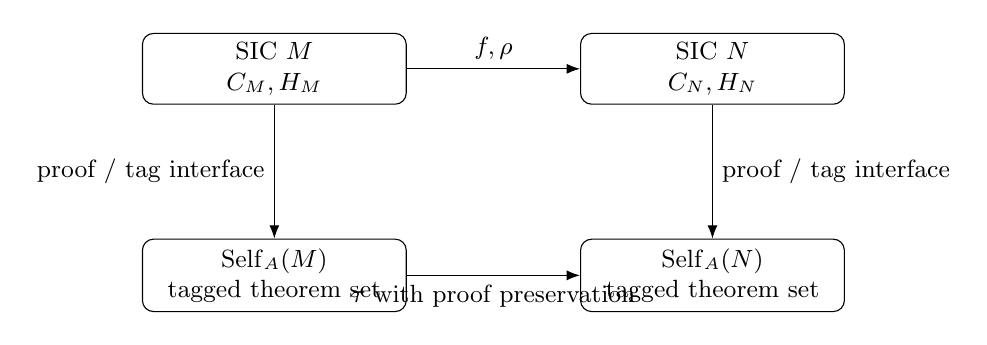
\begin{tikzpicture}[node distance=1.7cm and 2.2cm,>=Latex,every node/.style={font=\small},b/.style={draw,rounded corners,minimum width=3.35cm,align=center,minimum height=.85cm}]
\node[b] (s1) {SIC $M$\\$C_M,H_M$};
\node[b,right=of s1] (s2) {SIC $N$\\$C_N,H_N$};
\node[b,below=of s1] (t1) {$\Self_A(M)$\\tagged theorem set};
\node[b,below=of s2] (t2) {$\Self_A(N)$\\tagged theorem set};
\draw[->] (s1)--node[above]{$f,\rho$} (s2);
\draw[->] (s1)--node[left]{proof / tag interface} (t1);
\draw[->] (s2)--node[right]{proof / tag interface} (t2);
\draw[->] (t1)--node[below]{$\tau$ with proof preservation} (t2);
\end{tikzpicture}
\caption{Clocked state simulation is the top arrow; the bottom arrow does not exist without independent language and certificate hypotheses.}
\end{figure}

\subsection{A genuine transfer theorem}
\begin{theorem}[Tag- and proof-preserving clocked transfer]\label{thm:transfer}
Suppose $M\clksim N$ via $(f,\rho)$, and suppose there is an admissible language translation $\tau$ such that (i) $f(A_M)=A_N$, and (ii) whenever $p=C_M(A_M,m)$ and $\psi\in p\cap\SD_M$, the translated formula $\tau(\psi)$ belongs to $f(p)\cap\SD_N$. Then $M\sas N$ and $\lev(M)\le\lev(N)$. If, in addition, an accepted source certificate of $\psi$ always translates to an accepted target certificate for $\tau(\psi)$, the transfer preserves certified self-description.
\end{theorem}
\begin{proof}
Let $\psi\in\Self_A(M)$. Then $\psi$ appears at some stage $m$ on input $A_M$. By (ii), $\tau(\psi)$ belongs to $f(C_M(A_M,m))=C_N(f(A_M),\rho(m))=C_N(A_N,\rho(m))$, and belongs to $\SD_N$. It therefore lies in $\Self_A(N)$. This proves $\tau[\Self_A(M)]\subseteq\Self_A(N)$, and hence $M\sas N$; Theorem~\ref{thm:monotone} gives the level inequality. The final assertion follows from the additional verifier translation hypothesis for each certified source formula.
\end{proof}
\begin{remark}
The membership-observation assumption (ii) is not implied by clocked simulation: the latter preserves sets as abstract machine states under an injective $f$ but does not assert that an image state contains a translated formula. The certificate hypothesis is similarly independent. This is precisely the extra interface required to move from machine simulation to reflection preservation.
\end{remark}

\section{Two depths, two time scales, and their relation}
The word \emph{depth} refers to several inequivalent quantities. A reflection index counts nested provability assertions; a proof horizon counts primitive inference steps; and discovery time records when the particular ATP emits a target. These are not interchangeable.
\begin{definition}[Reflection discovery stage]
For $k\ge0$, set
\[
t_M(k):=\min\{m\ge1:\theta_k^M\in C_M(A_M,m)\},
\]
with $t_M(k)=\infty$ if the set is empty. Put $h_M(k)=h_F(A_M,\theta_k^M)$ for minimum total primitive-inference applications, and let $d_M(k)$ be the minimum \emph{dependency depth}, meaning the minimum possible longest chain of primitive inference applications in a derivation of $\theta_k^M$. Define the \emph{verified first stage} $t_M^V(k)$ similarly with membership replaced by the existence of an accepted proof certificate by that stage.
\end{definition}
\begin{proposition}[Clocked time transport under observational alignment]\label{prop:time}
Suppose $M\clksim N$ via $(f,\rho)$, $f(A_M)=A_N$, and a language translation $\tau$ sends each $\theta_k^M$ to $\theta_k^N$ and satisfies, on states of the compared trajectories,
\[
\theta_k^M\in p \quad\Longleftrightarrow\quad \theta_k^N\in f(p).
\]
Then for every $m\ge1$,
\[
\theta_k^M\in C_M(A_M,m)\quad\Longleftrightarrow\quad
\theta_k^N\in C_N(A_N,\rho(m)).
\]
Consequently $t_M(k)=\infty$ iff $N$ never contains $\theta_k^N$ at the sampled times $\rho(m)$; if $t_M(k)<\infty$, then $t_N(k)\le\rho(t_M(k))$.
\end{proposition}
\begin{proof}
Apply the simulation equation at $p=A_M$ and the membership-alignment hypothesis. If $t_M(k)$ is finite, the right-hand membership holds at stage $\rho(t_M(k))$, establishing the bound. If the source membership never occurs, neither can the target membership at a sampled time, by the biconditional.
\end{proof}
\begin{remark}[Why the reverse discovery-time equality is not asserted]
If $\rho$ skips stages, a target event could occur in an unsampled interval. For a SIC, monotone states mean that a target event persisting to later stages will eventually be visible at a sampled stage because $\rho$ is unbounded. Under the membership biconditional, this extra SIC monotonicity upgrades the proposition's sampled-time nonoccurrence to $t_N(k)=\infty$; it does \emph{not} produce a general numerical equality of first-stage times.
\end{remark}
\begin{proposition}[Rule-driven bound on awareness inference depth]\label{prop:lower}
If $M$ is rule-driven and $t_M(k)<\infty$, then
\[
d_M(k)\le t_M(k)-1.
\]
No analogous bound on the \emph{total} inference count $h_M(k)$ follows without a bound on the amount of work a stage may perform.
\end{proposition}
\begin{proof}
Induct on stages. Each stage-one formula is a premise and has derivation depth zero. If a new formula appears at stage $m+1$, the rule-driven condition supplies a legal finite-arity rule whose premises are already present at stage $m$. By the induction hypothesis, the premises have derivation depth at most $m-1$; attaching the final rule yields depth at most $m$. This proves the displayed bound. A stage can add many independent formulas or use a large proof DAG, so it need not bound the total number of inference applications.
\end{proof}
\begin{example}[Large awareness height, small or large work]
The premise-handed machines of Theorem~\ref{thm:finite} have arbitrarily large $\lev(M_n)=n$ while every proved reflection sentence is available at stage one, so high level need not entail discovery effort. In the rule-driven $\omega$ machine, $t_R(k)\le k+2$ on the designated input; delaying legal applications can make the same reflection assertions appear much later. The logical depth and operational discovery time thus answer different questions.
\end{example}

\section{Nondeterminism: may, must, and the fairness boundary}
The deterministic $C$ of a SIC already specifies a unique stage-indexed output for each input. A branching system requires additional data; it is not obtained by merely changing the word ``deterministic'' in the simulation definition.
\begin{definition}[Branching ATP presentation; proposed extension]
A branching ATP is a labeled transition system $\mathcal B=(Q,q_0,\longrightarrow,L,V)$ with rule-complete states $Q$, initial state $q_0$, transition relation $\longrightarrow\subseteq Q\times\Lambda\times Q$, a label $L(q)\subseteq\Sent(L_M)$ of accepted formulas, and a verifier interface $V$. A history is a finite or infinite legal labeled path from $q_0$. The allowed policy and fairness class are part of the presentation.
\end{definition}
\begin{definition}[May and must reflection levels]
For each $k$, \emph{may-$k$} means some finite legal accepted history reaches a state containing $\theta_k$. \emph{must-$k$}, relative to a declared fairness class $\mathcal F$, means every maximal fair history eventually reaches such a state. These have distinct quantifiers:
\[
\exists h\in\Hist(\mathcal B)\ \theta_k\in L(\operatorname{last}(h)),\qquad
\forall h\in\mathcal F\ \exists m\ \theta_k\in L(h_m).
\]
\end{definition}
\begin{example}[May without must]
A controller can choose either (i) a branch generating $\theta_0$ in one move or (ii) an infinite legal branch that never emits it. Then may-Level 1 holds but must-Level 1 fails if both branches are fair/admissible. An exploration procedure that eventually serves every enabled branch under a fair dovetailing policy changes the must-analysis; the fairness policy must therefore be frozen before any claim.
\end{example}
\begin{theorem}[Bisimulation preserves finite certified reflection traces]\label{thm:bisim}
Let $\mathcal B$ and $\mathcal B'$ be branching ATPs with a relation $R\subseteq Q\times Q'$ containing their roots. Suppose (i) $R$ preserves the reflected formula labels under an admissible $\tau$, (ii) it is a strong labeled bisimulation, and (iii) verifier-acceptance status of attached certificates is preserved. Then every finite accepted history in one system has a matching accepted history of equal length in the other, with the same sequence of translated reflection observations. Consequently each finite may-$k$ property is preserved in both directions.
\end{theorem}
\begin{proof}
Induction on history length. At the root the state labels and acceptance observations agree by (i) and (iii). A matching outgoing edge exists by strong bisimulation, with successors in $R$. Repeat inductively. The converse direction uses the reverse matching clause. A finite history witnessing may-$k$ therefore translates into a finite history witnessing may-$k$ in the other system.
\end{proof}
\begin{remark}[Must-preservation is conditional]
For all-fair-history claims, one additionally needs infinite-path matching and a fair-history correspondence. A finite-trace theorem alone does not transport fairness or eventual settlement, and it does not assert equality of runtime costs.
\end{remark}

\section{History, provenance, and safe compression}
Tenneson's later history-geometric work distinguishes complete execution histories from current states and from the certificates reconstructed from those histories. Self-awareness is sensitive to precisely those distinctions: proving a statement about a previous proof can require information the current theorem set alone has forgotten.
\begin{definition}[Certified reflective history]
A certified reflective history is a finite sequence
\[
h=(q_0\xrightarrow{a_1}q_1\xrightarrow{a_2}\cdots\xrightarrow{a_m}q_m;\,\Pi_h),
\]
where $\Pi_h$ records provenance for every accepted self-descriptive formula. In particular, for each accepted $\Prov(\Mtag,\qname{\varphi})$, the record identifies the referenced proof claim and what verifier, if any, accepted it. This is a \emph{record format}, not an assertion that any source ATP currently implements it.
\end{definition}
\begin{definition}[Future-complete reflective quotient]
A relation $R$ on operational states is \emph{reflectively future-complete} if it preserves target, certified outcome, reflection label, and verifier-acceptance observations and is a labeled strong bisimulation for the future legal transitions. An accepted weighted edge must match an edge of identical primitive cost when weighted cost preservation is claimed.
\end{definition}
\begin{theorem}[Conditional reflective history quotient]\label{thm:quot}
Let $q:Q\to Q/R$ be a quotient by a reflectively future-complete relation. If all relevant states are reachable in the declared transition system and every labeled edge in the quotient lifts to an edge from every representative with the same primitive weight and acceptance label, then:
\begin{enumerate}[label=(\roman*)]
\item the set of finite certified reflection observation strings from each state is preserved by quotienting;
\item every reachable certified reflection target in the original graph is reachable in the quotient, and conversely from every representative of the corresponding quotient class;
\item the infimum of primitive path costs to such a target is unchanged whenever edge weights are nonnegative and the target predicate is constant on classes.
\end{enumerate}
\end{theorem}
\begin{proof}
For (i), use induction on finite histories and both bisimulation clauses; each step preserves the label and the verifier observation. For (ii), specialize to histories whose final label contains the certified target. For (iii), every original path maps to an equal-weight quotient path, so the quotient infimum is no larger. Conversely, the lifting hypothesis allows a quotient path to be constructed from any chosen representative with exactly the same edge weights; thus the original infimum is no larger. These inequalities prove equality.
\end{proof}
\begin{remark}[Compression is not automatically safe]
If the quotient retains only the set of formulas but forgets which certificate validated a $\Prov$ claim, it may merge histories whose future accepted actions differ. Such a quotient can preserve ordinary theoremhood while changing reflection histories. If verification or BANK lookup has additional nonprimitive computational cost, the theorem does not preserve that charge unless it too is recorded and matched.
\end{remark}
\begin{figure}[htbp]\centering
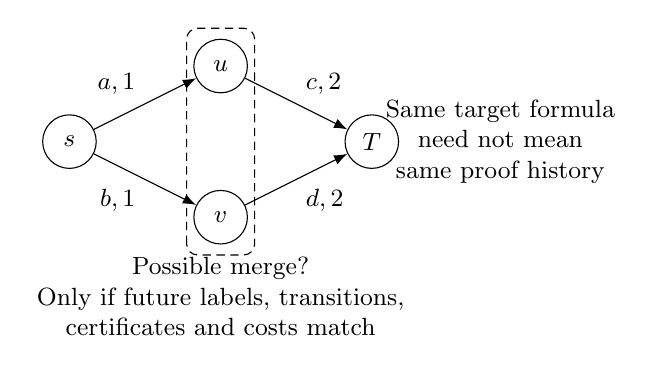
\begin{tikzpicture}[>=Latex,scale=.96, every node/.style={font=\small},q/.style={circle,draw,minimum size=.68cm,inner sep=2pt}]
\node[q] (a) at (0,1.4) {$s$}; \node[q] (b) at (2,2.4) {$u$};\node[q] (c) at (2,.4) {$v$};\node[q] (t) at (4,1.4) {$T$};
\draw[->] (a)--node[above left]{$a,1$}(b);\draw[->](a)--node[below left]{$b,1$}(c);
\draw[->](b)--node[above right]{$c,2$}(t);\draw[->](c)--node[below right]{$d,2$}(t);
\draw[densely dashed,rounded corners] (1.55,-.1) rectangle (2.45,2.9);
\node[align=center] at (2,-.65) {Possible merge?\\Only if future labels, transitions,\\certificates and costs match};
\node[align=center] at (5.7,1.4) {Same target formula\\need not mean\\same proof history};
\end{tikzpicture}
\caption{Coterminal paths need not be reflectively interchangeable. The dashed grouping is a candidate, not an automatically valid quotient.}
\end{figure}

\section{A worked model: a prover that proves its own kind}
We now give a small nontrivial toy case end-to-end. Fix an $xyz$ calculus containing the syntactic sentence $p:=\operatorname{ATP}(\langle K\rangle)$ and a premise $a$ expressing a formal specification token. Let $A_K=\{a\}$ and add only the unary inference $a\mapsto p$. Let $K$ be the rule-driven SIC from Example~\ref{ex:derived}; by direct computation,
\[
C_K(A_K,1)=\{a\},\qquad C_K(A_K,m)=\{a,p\}\quad(m\ge2).
\]
It follows that $p\notin A_K$ but $K\vdash_A p$ and the primitive-inference horizon is $h_F(A_K,p)=1$. The first discovery stage is $t_K(0)=2$. A verifier that checks the single rule application certifies $A_K\vdash_F p$.

If $\langle K\rangle$ faithfully denotes that rule-driven SIC and the predicate $\operatorname{ATP}$ is interpreted to include this specified class, the certificate is a true formal self-description relative to the declared semantics. If instead someone changes the predicate interpretation so that $\operatorname{ATP}(\langle K\rangle)$ is false, the unchanged syntactic proof is no longer a truthful self-description. Thus the formal certificate and its semantic application are different obligations.

The machine does \emph{not} prove $\theta_1=\Prov(\langle K\rangle,\qname p)$ unless a legal rule or premise supplies it. It has Level 1 but not Level 2. If we add $p\mapsto\theta_1$ then it derives Level 2 at stage 3. If the antecedent $p$ is accepted by the original verifier and the new reflection predicate correctly refers to $K$'s output relation, the new statement is justified. One can continue finitely many steps without claiming that the system has an unrestricted decision procedure for its own correctness.

\paragraph{Why the example is nondegenerate but modest.} The result was not handed as a hypothesis, and a verifier can check the derivation. The construction relies on a declared bridge axiom from $a$ to the claim of being an ATP. It does not make the machine aware of the entirety of its state-transition table, its future halting behavior, its proof efficiency, or its phenomenology.

\section{Cooperative ATPs and AMLD-style self-description}
The source two-page manuscript discusses individual ATPs, not a running multi-agent laboratory. A cooperative extension can be formulated without pretending that the original definitions already prove it.
\begin{definition}[Typed reflective cooperative state; proposal]
For a cooperative verifier-gated ATP architecture, let its accepted operational state contain worker states, scheduler state, an object-level BANK, a metatheoretic BANK, a provenance ledger, and a certified settlement record. A proposed self-description of the architecture is a statement $\psi(\langle\mathcal A\rangle)$ whose declared subject is the \emph{global architecture}, not automatically any individual worker.
\end{definition}
A proof deposited by worker $P$ that $P$ is an ATP is not a proof that the whole federation $\mathcal A$ is an ATP, and a claim that a worker has proved $\varphi$ is not a theorem about the whole federation unless a typed bridge axiom and verifier certify the relationship. The distinction becomes especially important when different roles operate over different metatheories.
\begin{proposition}[Conservative self-theory BANK growth; conditional]
Suppose an accepted object-level BANK sequence $B_0\subseteq B_1\subseteq\cdots$ satisfies $B_{i+1}\subseteq\Con_F(B_i)$ for each $i$, with sound finite certificates. Then for every $i$,
\[
\Con_F(B_i)=\Con_F(B_0).
\]
Therefore the set of \emph{logically derivable} self-descriptive sentences relative to $F$ does not change under such deposits, though the explicit-premise proof horizon and realized discovery costs may change.
\end{proposition}
\begin{proof}
Monotonicity gives $\Con_F(B_i)\subseteq\Con_F(B_{i+1})$. Since $B_{i+1}\subseteq\Con_F(B_i)$, idempotence of consequence yields the reverse inclusion. Induct on $i$.
\end{proof}
\begin{remark}[Do not confuse mathematical output with experience]
The fact that an architecture formally proves a sentence about its own rule-complete state establishes a typed theorem only. ``Self-awareness'' in this manuscript is a technical, graded property of names and proofs, not an assessment of subjectivity, general intelligence, autonomy, or personhood.
\end{remark}

\section{Tegmark's self-aware substructures: a controlled comparison}
The original draft mentions Tegmark's self-aware substructures (SAS) as motivation. In the formal setting, introducing a unary predicate $\operatorname{SA}$ permits the sentence $\operatorname{SA}(\Mtag)$. One may define a \emph{syntactic Tegmark-style condition} by $M\vdash_A\operatorname{SA}(\Mtag)$.

\begin{proposition}[The self-ascription criterion is underdetermined]
The syntactic Tegmark-style condition can hold of a machine whose $C$ is stationary and whose $\operatorname{SA}$ sentence was supplied as an initial hypothesis. Therefore that condition alone does not imply rule-driven discovery, correct introspection, or nontrivial computational behavior.
\end{proposition}
\begin{proof}
Let $Y=\{q\}$, $q=\operatorname{SA}(\Mtag)$, $A_M=\{q\}$, $C(\Gamma,m)=\Gamma$, and $H=0$. The system is a SIC and emits $q$ at stage one, but performs no new derivation.
\end{proof}
A richer mathematical refinement distinguishes the mere assertion $\operatorname{SA}(\Mtag)$ from the following evidence: faithful designation; a correctly interpreted self-descriptive predicate; a legal derivation from premises not containing the target; an accepted verifier record; and a quantified hierarchy of correctly supported reflection assertions.

The inference from a formal self-ascription to phenomenological consciousness is \emph{not} licensed. Nor is the opposite inference, that the mathematical theory disproves consciousness. The formal structure was selected to address a narrower, testable question.

\section{What has been shown, what has not, and future research}
\subsection{The proof ledger}
\begin{center}\small\begin{tabularx}{\textwidth}{@{}p{.37\textwidth}p{.19\textwidth}X@{}}\toprule
Claim & Status & Required qualification \\\midrule
$\Self_A(M)=\Th_M(A_M)\cap\SD_M$ & Definition & Fixed subject grammar and designated input \\
Reflection formulas are distinct & Proved & Injective quotation and predicate distinction \\
Cumulativity of levels & Proved, conditional & Provability soundness \\
All finite levels exist & Proved & Hypothesis-handed toy witnesses \\
A rule-driven $\omega$ witness exists & Proved in idealized model & Infinite unary rule schema; operational reading of $\Prov$ \\
$\sas$ is a preorder; levels monotone & Proved & Admissible translations \\
Bare $\clksim$ preserves awareness & False in general & Names and proofs are not in SIC simulation axioms \\
Verified clocked transfer & Proved, conditional & Tag, theorem, verifier and observation alignment \\
Nondeterministic may-level preservation & Proved, conditional & Strong labeled bisimulation and verifier preservation \\
History quotient preserves primitive costs & Proved, conditional & Weighted lifting and cost-preserving bisimulation \\
Any actual human/machine is conscious & Not addressed & Outside the chosen formal semantics \\
\bottomrule\end{tabularx}\end{center}

\subsection{Open problems}
\begin{question}[Intrinsic awareness, not just inherited axioms]
What is the weakest nondegeneracy condition under which $\theta_0$ is derived from a certified specification rather than inserted into the premises? Can such a condition be preserved under an admissible self-theory equivalence?
\end{question}
\begin{question}[Complete invariants]
What invariants, beyond $\lev(M)$, classify the fibers of $D_{\mathrm{SA}}$? Are distinct reflective spectra with the same supremum necessarily separable by admissible translations?
\end{question}
\begin{question}[Simulation geometry]
For which classes of ATPs is every clocked simulation augmentable to a tag- and certificate-preserving self-awareness translation? If not, characterize the minimal missing labels.
\end{question}
\begin{question}[Reflection and semantic truth]
What representability assumptions are needed before the primitive $\Prov$ becomes a genuine arithmetized provability predicate? Under which consistency and expressibility hypotheses do G\"odel, L\"ob, or Tarski limitations apply?
\end{question}
\begin{question}[Quantitative self-awareness]
Can one identify resource-sensitive bounds relating the reflection index, inference depth, total proof work, scheduler-robust settlement, and cost of checking an accepted self-description?
\end{question}
\begin{question}[Nondeterministic fairness]
What is the weakest simulation relation preserving must-reflection levels under fair scheduling? How do the answers change for probabilistic or adversarial environments?
\end{question}
\begin{question}[Minimal certified history]
What is the smallest future-complete state representation that preserves certified reflection observations, legal continuations, and charged settlement costs? Can a significant reduction be exhibited on an actual prover trace?
\end{question}
\begin{question}[Transfinite levels]
A provability-sound level $\omega$ machine proves every sentence in the \emph{finite} reflection ladder. A further ordinal hierarchy requires an explicit limit-stage sentence or schema, an admissible naming construction, and a semantics for reflection at a limit. Does a coherent useful extension exist under soundness constraints?
\end{question}
\begin{question}[Empirical validation]
Given a fixed benchmark, frozen theorem library, proof checker, and charged resource budget, do reflective tags or backward-history certificates improve performance compared with an otherwise identical ATP lacking those resources? This is an experimental question, not settled by the existence theorems.
\end{question}

\section{Conclusion}
The mathematics of self-awareness begins at an unusually modest point: a formal machine must be named in its own language and must derive a sentence belonging to a declared class of statements about that name. From this point the theory has substantive structure. It distinguishes the act of naming from the truth of a self-ascription; it measures nested provability by a reflection sequence; it proves cumulativity under soundness and attainment of $\omega$ under necessitation; and it separates the simulation preorder on SIC behavior from a second preorder on preserved self-theory.

The sharpest warning is also the most productive design principle: \emph{a simulation of a machine does not automatically simulate its account of itself}. To transfer reflective information, the embedding must carry names, syntax, proof acceptance, and relevant histories in addition to stages and halting observations. This is where proof-search geometry and certified computation histories become mathematically useful rather than merely suggestive.

The resulting formalism offers a theory of \emph{certified self-description}. It is not a complete theory of consciousness, not a proof of universal self-knowledge, and not an empirical claim about existing software. Its value lies in making precise which obligations would have to be proved next.

\section*{Source note and references}
\addcontentsline{toc}{section}{Source note and references}
\begin{enumerate}[label={[\arabic*]},leftmargin=2.6em]
\item \textless{}Brian Tenneson\textgreater{}, \emph{Self-Awareness}, original two-page draft supplied with this request (title, abstract, Definitions 2.1--2.5, eight development directions). Historical source; preserved conceptually rather than overwritten.
\item \textless{}Brian Tenneson\textgreater{}, \emph{Depths of a Simulation \& Formalized Self-Awareness}, corrected core reproduced in \emph{Certified History--Rendezvous Geometry}, research draft 0.2, October 28, 2026. Source for the SIC axioms, clocked simulation, corrected syntactic $\SD_M$ convention (C42), corrected admissible translation (C43), and reflection hierarchy.
\item \textless{}Brian Tenneson\textgreater{}, \emph{Certified History--Rendezvous Geometry: A Three-Theory Intertwining}, research draft 0.2, October 28, 2026. Used here only for the separate history/certificate and safe-quotient perspective; no unconditional performance conclusion is transferred from it.
\item Max Tegmark, work on self-aware substructures and the mathematical universe, cited as conceptual motivation in the source manuscript. No physical or phenomenological claim is deduced from that discussion.
\end{enumerate}
\end{document}